\documentclass[11pt,a4paper]{article}

%
% $Id: howtobuild.tex,v 1.14 2006/04/25 14:20:24 schnelle Exp $
%

\usepackage[latin1]{inputenc}
\usepackage{graphics}
\usepackage{graphicx}
\usepackage{url}
\usepackage{listings}
\usepackage{xcolor}
\usepackage{jvoicexml}
\usepackage[pdftex, citecolor=black, urlcolor=black,
linkcolor=black, colorlinks=black, colorlinks=true,
 bookmarksopen=true]{hyperref}
\include{version}

\title{How to build JVoiceXML \jvxmlversion}
\author{Dr. Dirk Schnelle-Walka}
\email{dirk.schnelle@jvoicexml.org}
\date{\today}

\begin{document}

\pagestyle{empty}
\lstset{language=Java,language=XML,
        backgroundcolor=\color{lightgray},
        basicstyle=\small,
        numbers=left,
        numberstyle=\tiny,
        breaklines=true, 
        breakatwhitespace=false, 
        flexiblecolumns,
        stepnumber=5}

\maketitle

\pagestyle{headings}

\tableofcontents

\newpage

\begin{abstract}
This documents describes the steps you have to perform, when you want
to build JVoiceXML or develop code for the JVoiceXML project. It gives
information about the requirements of your development environment 
and our coding conventions.
\end{abstract}

\section{Introduction}
\label{sec:introduction}

JVoiceXML is a free VoiceXML~\cite{w3.org:voicexml} implementation written in 
the JAVA programming language. It offers a library for easy VoiceXML
document creation and a VoiceXML interpreter to process 
VoiceXML documents using JAVA standard APIs such as JSAPI~\cite{sun:jsapi} and
JTAPI~\cite{sun:jsapi}.

VoiceXML was previously hosted at SourceForge~\cite{sourceforge} as an open source project
under \url{http://sourceforge.net/projects/jvoicexml/}. Now, the code hase been made
available at GitHub at \url{https://github.com/JVoiceXML/JVoiceXML}.
You find everything that is related to this project att GitHub.

This document refers to UNIX and Windows systems. JVoiceXML will work 
any other operating systems that support Java 8, too.

Nobody is perfect, so you may find some errors or small things to correct.
Please let me know if you think you found something that should be written
differently.

\section{Copyright}
\label{sec:copyright}

JVoiceXML uses the GNU library general public license~\cite{gnu:lgpg}. 
This is mentioned in all our source files as a unique header, see
section~\ref{sec:code-conventions}.
You can find a copy in the file \texttt{doc/copying.xhtml} in the \$\{JVOICEXML\_HOME\}
directory. This means that you are allowed to use JVoiceXML
library in your commercial programs. If you make some nice
enhancements it would be great, if you could share them
with us, e.g. by a pull request, so that we can make it available to the community.

JVoiceXML is distributed in the hope that it will be useful,
but WITHOUT ANY WARRANTY; without even the implied warranty of
MERCHANTABILITY or FITNESS FOR A PARTICULAR PURPOSE. See the GNU
Library General Public License for more details.

You should have received a copy of the GNU Library General Public
License along with this library; if not, write to the Free
Foundation, Inc., 59 Temple Place, Suite 330, Boston, MA  02111-1307  USA

\section{Download the Source Code}

\subsection{Download the Source Archive}

You can download a the source code for the available releases from 
\url{https://github.com/JVoiceXML/JVoiceXML/releases}. The recommended way is to
use the Git repository as described in the following sections. 

\subsection{Git Repository}
\label{sec:git-repository}

If you want to stay at the current state of development you have to use
the Git repository from GitHub\footnote{\url{http://github.com}}. This is also
the preferred way. Some older stuff is still at Source Forge~\cite{sourceforge}
but this is no longer actively maintained.

This section describe the parameters to access the Git repository 
using the command line. Feel free to grab the required parameters from
this description and feed your favorite tool with them.

\begin{lstlisting}
git clone  https://github.com/JVoiceXML/JVoiceXML.git
\end{lstlisting}

This will check out all projects of JVoiceXML
into the folder \texttt{JVoiceXML}. 

A screenshot from a checkout in eclipse is shown in
figure~\ref{fig:eclipse-projects}.
\begin{figure}
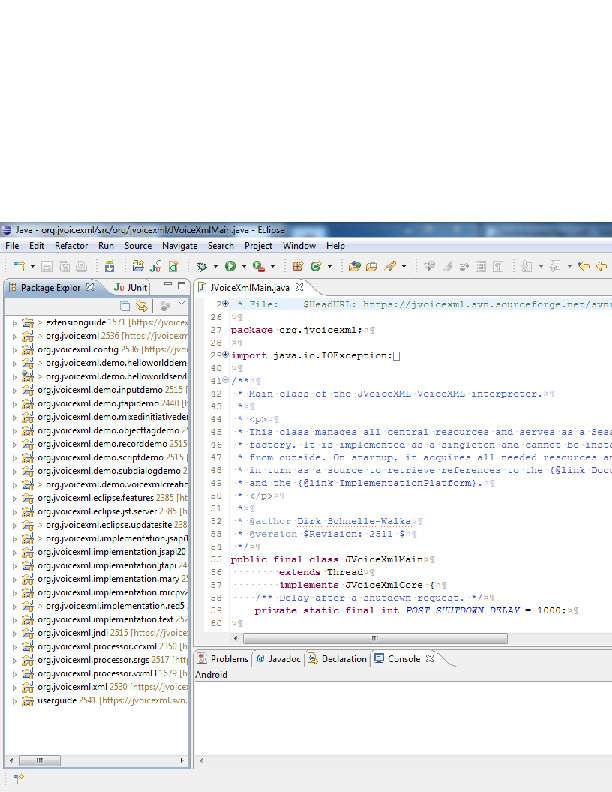
\includegraphics[width=\linewidth]{eclipse-projects.png}
\caption{Eclipse project overview of JVoiceXML}
\label{fig:eclipse-projects}
\end{figure}

\textbf{Note:} UNIX file and directory names are case sensitive.

All projects follow the convention that they have the same name as the jar
that will be produced when bundling them. For instance, the jar \lstinline{org.jvoicexml.xml.jar}
is built by the project \lstinline{org.jvoicexm.xml}.

\section{Required Software}
\label{sec:required-software}

Since JVoiceXML is written in JAVA you will at least need a
JAVA compiler, see section~\ref{sec:ide}, an editor or preferably a JAVA
IDE, see section~\ref{sec:ide}, and Gradle, to build the
binaries. All used third party libraries can be downloaded from the CVS, SVN or
comparable repository or from their home pages. The file
\texttt{doc/libraries.xhtml} contains a list of all used libraries.


\subsection{IDE}
\label{sec:ide}

JVoiceXML is being developed using eclipse 4.6, but you can use the IDE of your
choice to edit the sources and compile the binaries. You can even use a simple
text editor to perform this job. Nevertheless there are some restriction that
you cannot work around.

Your IDE must support

\begin{itemize}
\item JavaSE 8
\item Gradle 6.9.1
\end{itemize}

\subsection{JAVA}
\label{sec:java}

Parts of the code of JVoiceXML are using features from the JAVA 8 API, so that
you will need at least JSE 8 to compile the code. You can download it
for free from \url{http://oracle.com/technetwork/java/javase/downloads/index.html}.
While newer Java versions are available they are not proven to be supported.

In case you are using another IDE, you will have to manually adapt
the required library settings, e.g. gor code completion. The dependencies to all
libraries are listed in \lstinline{JVOICEXML_HOME/doc/libraries.xhtml}.


\subsubsection{Eclipse settings}
\label{sec:eclipse}

If you are not using eclipse as your favorite IDE, you may ignore this section.
We are using the \emph{Eclipse IDE for Java EE Developers}
for the development of JVoiceXML. The Git repository contains the eclipse
project settings. This way, there is no need to import the
project into eclipse. The project settings will be detected 
automatically when you checkout the projects. However you are requested to configure the execution
environment development for Java 8 \emph{JavaSE-1.8} to point to a valid JDK.
The use of execution environments makes the development independent of the
used version of the Java 8 SDK.

A screenshot for a possible configuration is shown in
figure~\ref{fig:eclipse-execution-environments}.
\begin{figure}
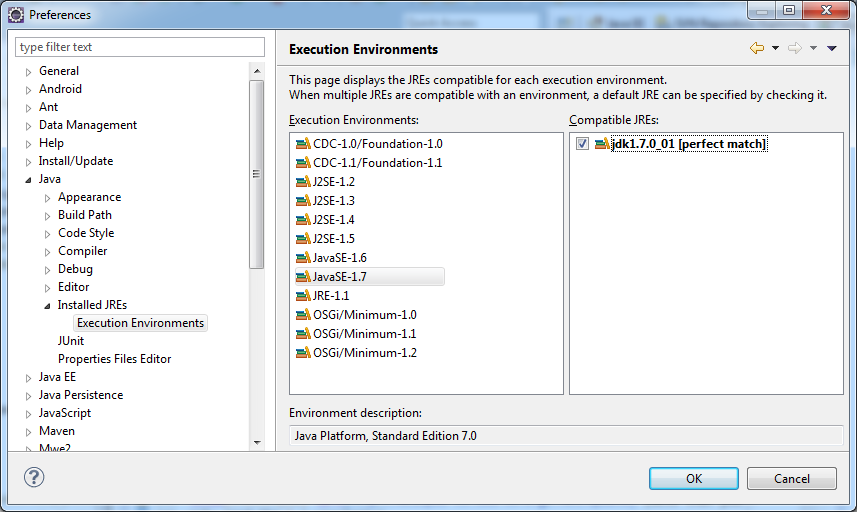
\includegraphics[width=\linewidth]{eclipse-execution-environments}
\caption{Configuration of the Java 8 Execution Environment in eclipse}
\label{fig:eclipse-execution-environments}
\end{figure}

\paragraph{Required Eclipse Plug-ins for Development}

The development of JVoiceXML relies on some plug-ins that are not part of the
IDE. You will need to install the following eclipse plug-ins via the eclipse
Software Update mechanism.

Below is a list of the required update URLs.

\begin{description}
\item[Buildship] \url{https://projects.eclipse.org/projects/tools.buildship} for Gradle support
\item[Checkstyle] \url{http://eclipse-cs.sourceforge.net/update} (Note that you
only need the 5.x version)
\item[TeXlipse] \url{http://texlipse.sourceforge.net} (optional if you want to
edit the documentation) This will also require an existing \LaTeX installation.
\item[Gitflow] for Gitflow support (optional for contributors).
\item[Protocol Buffers Development Tools] \url{http://code.google.com/p/protobuf-dt/}
(optional if you want to edit the protobuf files in the sub project
\texttt{org.jvoicexml.mmi.events} or \texttt{org.jvoicexml.client.text})
\end{description}

However, the preferred way to install the plugins is via the eclipse market place.

\subsection{Gradle}
\label{sec:gradle}

JVoiceXML is being built by Gradle. It is recommended that
you use Gradle 6.9.1 as Gradle 7.0 is not yet supported.. 
If you don't have Gradle installed, you can download the current release
from \url{http://www.gradle.org}. This should not be necessary if Gradle is builtin
your IDE.

The build file allows you to override the settings by using a custom 
properties file \texttt{gradle.properties} in the \texttt{\$\{HOME\}/.gradle}
directory. This will be referred to as your \emph{your copy} later in this document.

Since almost all IDEs feature support for Gradle, at least with the help of plugins, it will be possible to
use your favorite IDE.


\subsubsection{Gradle Support for Eclipse}
\label{sec:gradle-eclipse}

The Gradle project files are usually named \texttt{build.gradle} and reside the 
project root folder as well as in the folders of the subprojects. 
In order to run an Gradle target from within
eclipse you can use the \emph{Gradle Tasks} view as shown in
figure~\ref{fig:eclipse-run-gradle}.
\begin{figure}
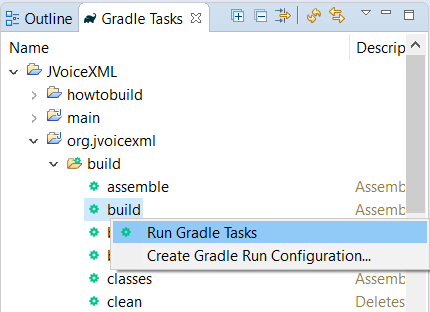
\includegraphics[width=\linewidth]{eclipse-run-gradle}
\caption{Run a Gradle tasks from within Eclipse}
\label{fig:eclipse-run-gradle}
\end{figure}

This view is part of Eclipse's Buildship integration for Gradle.

\subsection{Tomcat}
\label{sec:tomcat}

For the system test and for some demos you will need to have a servlet
container installed. We use Tomcat 8 for that purpose. You can download this
release from \url{http://tomcat.apache.org}.

This is not needed if you do not use the servlet based demos or want to run the
system test.

\subsection{\LaTeX}

The documentation is being written using \LaTeX. If you want to edit the
documentation you will need to install a \LaTeX system like MiKTeX
\url{http://miktex.org} for windows or tetex on Linux systems.

For Linux you will need the packages
\begin{itemize}
  \item texlive-latex-base
  \item texlive-fonts-recommended
  \item texlive-fonts-extra
  \item texlive-fonts-extra
\end{itemize}
This is not needed if you do not want to author the documentation or create a
distribution.

\section{Project Conventions}

JVoiceXML comprises several projects. Some of them are described in more
detail in the following section. All these projects follow some conventions
that should ease staying oriented.

The base namespace for all projects is \lstinline{org.jvoicexml}. Dependent 
projects may extend this namespace. For instance the namespace for the
XML library is \lstinline{org.jvoicexml.xml}.

The project names have the same name as the jar that they produce. This
makes it easier to find the project related to a specific Java archive.
For instance the project name for the XML library is
\lstinline{org.jvoicexml.xml}. It produces the jar
\texttt{org.jvoicexml.xml.jar}.
The drawback of this approach is that you will be confronted 
with a huge list of projects. The minimal set of projects
that are required to build JVoiceXML is marked in the list
given in section~\ref{sec:jvoicexml-core}.

The project names generally also reflect the overall architecture as shown in
figure~\ref{fig:main-components}.
\begin{figure}
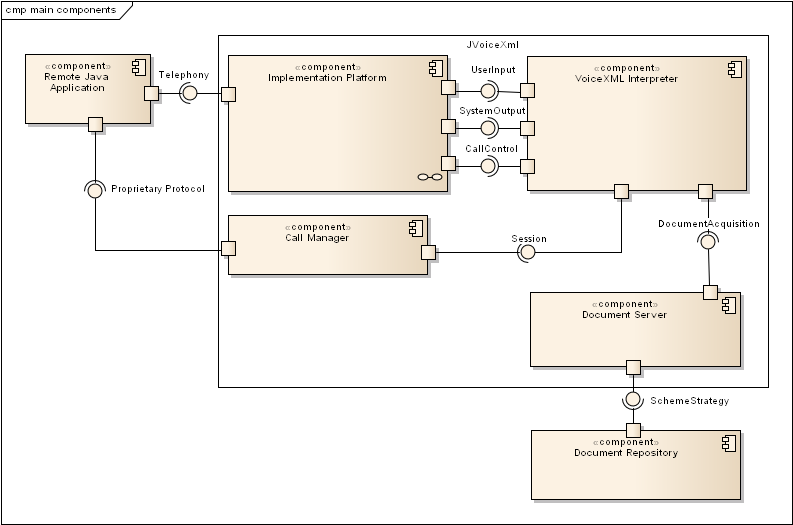
\includegraphics[width=\linewidth]{main-components.png}
\caption{JVoiceXML general architecture}
\label{fig:main-components}
\end{figure}
These components can be mapped to the packages as shown in
figure~\ref{fig:main-packages}. Specializations manifest as subpackages thereof.
For instance, the JSAPI 2.0 implementation platform resides in package 
\lstinline{org.jvoicexml.implementation.jsapi20} as a subpackage of
\lstinline{org.jvoicexml.implementation} (but in another project).
\begin{figure}
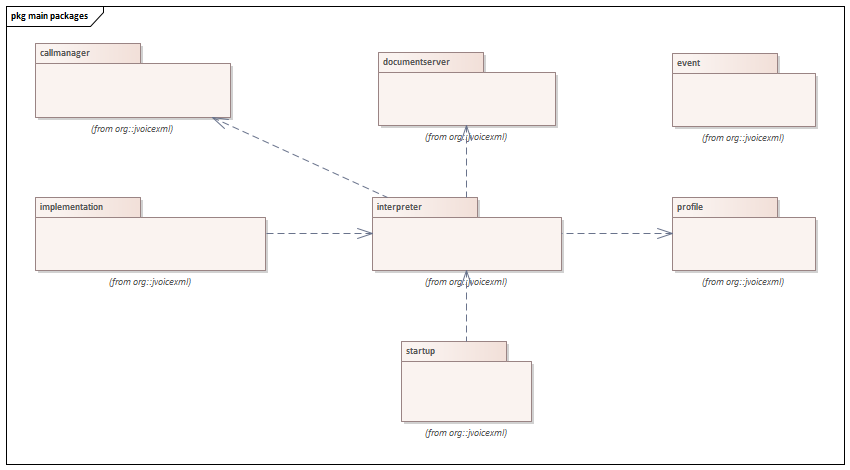
\includegraphics[width=\linewidth]{main-packages.png}
\caption{Main packages of JVoiceXML}
\label{fig:main-packages}
\end{figure}


Within a project the following directory structure applies as suggested by
Gradle

\begin{description}
\item[build] compiled binaries
\item[src/main/java] Java source code
\item[src/main/resources] Additional resource files to be integrated in the Jar
\item[src/main/config] Project specific configuration files
\item[src/test/java] JUnit tests and other tests.
\item[src/test/resources]  Additional resource files for the tests
\item[build.gradle] Gradle build file
\ref{sec:create-configuration})
\end{description}

Demo projects may have an additional folder \texttt{config} to hold
configurations settings. 

\section{JVoiceXML Core}
\label{sec:jvoicexml-core}

The core of JVoiceXML comprises the following sub-projects, also shown in~\ref{fig:core-projects}:
\begin{figure}
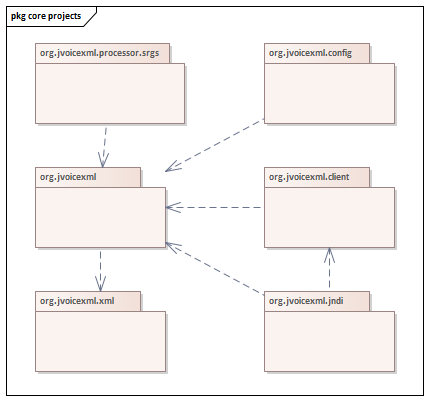
\includegraphics[width=\linewidth]{core-projects.png}
\caption{Core projects of JVoiceXML}
\label{fig:core-projects}
\end{figure}

\begin{description}
\item[org.jvoicexml] The core of the interpreter
\item[org.jvoicexml.config] JVoiceXML configuration based on spring
\item[org.jvoicexml.client] Client libraries to interacti with JVoiceXML
remotely.
\item[org.jvoicexml.jndi] JNDI support for JVoiceXML
\item[org.jvoicexml.srgs] SRGS processor (required)
\item[org.jvoicexml.xml] The JVoiceXML XML library (required)
\end{description}

The most convenient configuration setting is the one for \emph{JSAPI 2.0}. Here,
you will need to configure for the folloging projects:
\begin{itemize}
  \item org.jvoicexml
  \item org.jvoicexml.client
  \item org.jvoicexml.config
  \item org.jvoicexml.implementation.jsapi20
  \item org.jvoicexml.interpreter.datamodel.ecmascript
  \item org.jvoicexml.jndi
  \item org.jvoicexml.processor.srgs
  \item org.jvoicexml.profile.vxml21
  \item org.jvoicexml.xml
\end{itemize}
See also section~\ref{sec:implementation-jsapi20}.

A simple demo to test that implementation platform to start with is
\lstinline{org.jvoicexml.demo.helloworld}.

For a \emph{text} based configuration you will need
\begin{itemize}
  \item org.jvoicexml
  \item org.jvoicexml.client
  \item org.jvoicexml.client.text
  \item org.jvoicexml.config
  \item org.jvoicexml.implementation.text
  \item org.jvoicexml.interpreter.datamodel.ecmascript
  \item org.jvoicexml.jndi
  \item org.jvoicexml.srgs
  \item org.jvoicexml.profile.vxml21
  \item org.jvoicexml.xml
\end{itemize}
See also section~\ref{sec:text-implemenation-platform}

A simple demo to test that implementation platform is
\lstinline{org.jvoicexml.demo.text}.

\subsection{Project \texttt{main}}

This project is the core of the JVoiceXML browser and the central point of
building and configuring the environment.

\subsection{Project \texttt{org.jvoicexml}}

This project is the core of the Voice Browser.

\subsubsection{Creating a Configuration}
\label{sec:create-configuration}

There are several implementations for the implementation platform available
that reside in co-projects, refer to section~\ref{sec:git-repository}. Multiple
implementation platforms can be active at the same time. They will be activated at runtime
if the corresponding configuration file is found in the config folder.

The file \texttt{\$JVOICEXML\_HOME/gradle.properties} (see Apeendix \ref{sec:gradle-properties}) 
contains templates for all
the switches and settings that may be used to enable or disable certain
implementation platforms or adapt needed configuration settings.

This adaptation should be done via your local copy of this file in your
local copy of that content at \texttt{gradle.properties} in
\texttt{\$HOME/.gradle}.

Once you changed the settings cd to the main subproject and call
\begin{lstlisting}
gradle run
\end{lstlisting}
to start the Voice Browser.
and stopped it by
\begin{lstlisting}
gradle shutdown
\end{lstlisting}

Please do not stop the voice browser by \texttt{CTRL-C} or similar. It may occur
that some resources are not closed properly and may cause conflicts with the next
start of JVoiceXML. This is because it is not possible to properly shutdown the
RMI registry.

The \texttt{build.gradle} also contains a target to enable remote
debugging. It can be called by
\begin{lstlisting}
gradle runDebug
\end{lstlisting}
The code will be compiled using your current configuration and the start of the
voice browser will be delayed until you connect with a remote debugger. The
used server port is 12367. This allows to set breakpoints using your IDE and
debug JVoiceXML.

\subsubsection{The Main Build File}
\label{sec:main-build-file}

This section explains the most important targets of the main build file
\texttt{build.gradle} in the main subproject. All others build files from the
implementation platforms
are called from this central point. Just start gralde without any target specified
if you want to build everything. Call
\begin{lstlisting}
gradle tasks
\end{lstlisting}
to get an overview of the targets and their purpose.

\begin{description}
\item[clean]
Delete all compiled class files in the directory \emph{build}
and the jars that are created by the \emph{jar} target in the directory 
\emph{dist}.

\item[jar]
This target dcreates the jar files of your distribution.
If successful, you will find at minimum the following jar archives:
\begin{itemize}
\item org.jvoicexml.jar This jar file contains the core of JVoiceXML.
\item org.jvoicexml.xml.jar This jar contains all files that are required
to create and parse VoiceXML documents. This file is being build from the
project \texttt{org.jvoicexml.xml} which is described in
section~\ref{sec:org.jvoicexml.xml}.
\item org.jvoicexml,client.jar This jar contains the files needed to build
a client.
\item org.jvoicexml.jndi.jar JNDI support for JVoiceXML
\item org.jvoicexml.srgs
\item some other jars, depending on your configuration settings
\end{itemize}

\item[javadoc]
Create JAVADOC documentation from the JAVA files in the directory.
\item[run] Build all the configured implementation platforms
via \texttt{gradle.properties}, copy their configuration files into a
temporary configuration folder and start the JVoiceXML voice browser.
\item[shutdown] Remotely shutdown the JVoiceXML voice browser.
\item[distribution] Create a distribution for all subprojects.
\end{description}

Call
\begin{lstlisting}
gradle <target>
\end{lstlisting}
to run Gradle for the the given target.

The Gradle launch configurations for eclipse are part of the Git repository. They
are available as a shortcut in the run. A screenshot is shown in figure~\ref{fig:eclipse-launch}.
\begin{figure}
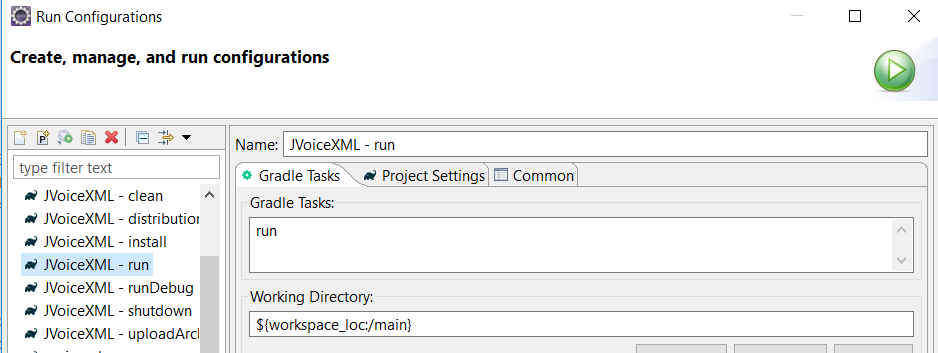
\includegraphics[width=\linewidth]{eclipse-launch.png}
\caption{Run configuration for JVoiceXML}
\label{fig:eclipse-launch}
\end{figure}

\subsection{Project \texttt{org.jvoicexml.config}}
\label{sec:org.jvoicexml.config}

This project provides a library to configure JVoiceXML based on the spring
framework.
This is not required at run time and can be replaced by custom
implementations, e.g. to embed JVoiceXML. However, it is required to build
JVoiceXML.

This project has to be build after the main project.

\subsection{Project \texttt{org.jvoicexml.xml}}
\label{sec:org.jvoicexml.xml}

This project provides an XML library to create and parse all VoiceXML related
XML languages like SRGSXML, PLS and SSML.

This project has to be build before the main project.

\subsection{Project \texttt{org.jvoicexml.srgs}}
\label{sec:org.jvoicexml.srgs}

This project provides an SRGS processor.

\section{Remote Java Applications}

Remote applications initate calls to the call manager to create a session in JVoiceXML
as shown in figure~\ref{fig:remote-application-access}. In turn ASR, TTS and telephony resources
are associated with this session that can be used to interact with the user in the created session.
\begin{figure}
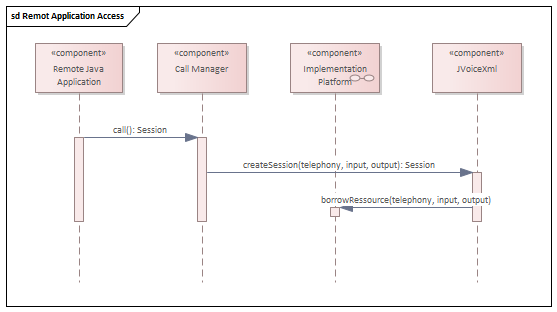
\includegraphics[width=\linewidth]{remote-application-access.png}
\caption{Remote application access}
\label{fig:remote-application-access}
\end{figure}

\subsection{Project \texttt{org.jvoicexml.client}}

This project contains the basic classes that are needed to implement a
client that can connect remotely to JVoiceXML. Depending on the used 
implementation platform additional client specializations may be needed
as detailed in section \ref{sec:implementation-platforms}.

\subsection{Project \texttt{org.jvoicexml.jndi}}
\label{sec:jndi}

This project provides JNDI support for JVoiceXML. Depending on the implementation platform this is not required at run
time but in order to build JVoiceXML.

JNDI offers remote access to JVoiceXML, e.g. the ability to run the
shutdown script or to run the demos. Conceptually, JNDI can be perceived as a JNDI
call manager. 

The project settings for this subproject can be adapted by the following 
properties in your copy of the \texttt{gradle.properties} file in the
\texttt{\${HOME}/.gradle} folder of the core project (see 
Appendix~\ref{sec:gradle-properties}):
\begin{description}
\item[JVOICEXMLJNDI\_REPOSITORY] id of the classloader repository that is used by the target implementation platform, e.g.
\texttt{text} for the text implementation plaform. 
\item[JVOICEXML\_JNDI\_PORT] Port number of the RMI registry
\item[JVOICEXMLJNDI\_CLASSERVER\_PORT] Port number of the classloader to enable automated cde download via RMI
\end{description}

The Gradle build script also adapts the settings in the
\texttt{jndi.properties} to the configured port. Make sure to also adapt
the \texttt{jndi.properties} in the demos or your application.

The repository entry must match the repository that you are using for your
client. Otherwise JVoiceXML will not be able to load the needed resources of
the server side. This limits the usage of JNDI to one platform only.

\subsubsection{Implementation Platform Configuration Files}

At runtime, JNDI support will be enabled if the following configuration file is found in the configuration
folder
\begin{itemize}
\item jvxml-jndi.xml
\end{itemize}

\section{Implementation Platforms}
\label{sec:implementation-platforms}

Implementation platforms comprise external resources, like
\begin{itemize}
  \item Telephony
  \item ASR
  \item TTS
\end{itemize}
as shown in figure~\ref{fig:implementation-platform}.
\begin{figure}
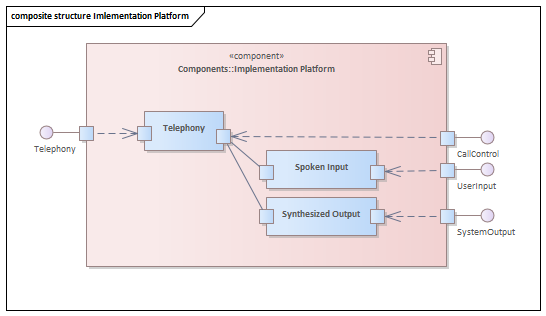
\includegraphics[width=\linewidth]{implementation-platform.png}
\caption{Implementation Platform}
\label{fig:implementation-platform}
\end{figure}

This section gives an overview of provided implementation platforms for JVoiceXML
and how to configure them.

\subsection{Project \texttt{org.jvoicexml.implementation.jsapi20}}
\label{sec:implementation-jsapi20}

This project contains a first draft of an implementation platform to enable
JSAPI 2.0 support for JVoiceXML. JSAPI 2.0 is being developed within the Java 
Community Process (JCP)~\cite{jcp} under JSR-113~\cite{jcp:jsr113}.

\subsubsection{Project Specific Configuration}

The project settings for this subproject can be adapted by the follow   ing 
properties in your copy of the \texttt{gradle.properties} file in the
\texttt{\${HOME}/.gradle} folder of the core project (see 
Appendix~\ref{sec:gradle-properties}):

\begin{description}
\item[JVOICEXML\_IMPLEMENTATION\_JSAPI20] A value of \texttt{true} will enable this implementation
platform and enable evaluation of the subsequent settings.
\item[JVOICEXML\_IMPLEMENTATION\_JSAPI20\_FREETTSSPHINX] A value of \texttt{true} will result in a
configuration that uses FreeTTS and Sphinx4 as speech engines and copy that configuration file to the temporary
configuration folder.
\item[JVOICEXML\_IMPLEMENTATION\_JSAPI20\_SAPI]  A value of \texttt{true} will result in a
configuration that uses the SAPI implementation as speech engines and copy that configuration file to the temporary
configuration folder.
\end{description}

\subsubsection{Implementation Platform Configuration Files}

At runtime, this platform will be enabled if one of the following configuration files is found in the configuration
folder
\begin{itemize}
\item jsapi-20-implementation.xml
\item jsapi-20-sapi-implementation.xml
\end{itemize}

\subsection{Project \texttt{org.jvoicexml.implementation.jtapi}}

This implementation platform provides telephony functionality based on JTAPI to
JVoiceXML. This implementation platform should be used together with other
implementation platforms like the JSAPI 2.0 implementation platform since it
does not have any speech functionality.

\subsubsection{Project Specific Configuration}

The project settings for this subproject can be adapted by the following
properties in your copy of the \texttt{gradle.properties} file in the
\texttt{\${HOME}/.gradle} folder of the core project (see 
Appendix~\ref{sec:gradle-properties}):
\begin{lstlisting}
JVOICEXML_IMPLEMENTATION_JTAPI = false
JVOICEXML_IMPLEMENTATION_JTAPI_SIP_PROVIDERNAME = net.sourceforge.gjtapi.raw.mjsip.MjSipProvider
JVOICEXML_IMPLEMENTATION_JTAPI_SIP_ADDRESS = 127.0.0.1:4246
JVOICEXML_IMPLEMENTATION_JTAPI_SIP_TERMINAL = sip:jvoicexml@127.0.0.1:4247
JVOICEXML_IMPLEMENTATION_JTAPI_SIP_PORT = 4246
JVOICEXML_IMPLEMENTATION_JTAPI_SIP_INPUTTYPE = jsapi20
JVOICEXML_IMPLEMENTATION_JTAPI_SIP_OUTPUTTYPE = jsapi20
\end{lstlisting}

\subsubsection{Implementation Platform Configuration Files}

At runtime, this platform will be enabled if the following configuration file is found in the configuration
folder
\begin{itemize}
\item mary-implementation.xml
\end{itemize}

\subsection{Project \texttt{org.jvoicexml.implementation.lightweightbml}}

This implementation provides support for BML JVoiceXML as a lightweight means to show an avatar

\subsubsection{Project Specific Configuration}

The project settings for this subproject can be adapted by the following 
properties in your copy of the \texttt{gradle.properties} file in the
\texttt{\${HOME}/.gradle} folder of the core project (see 
Appendix~\ref{sec:gradle-properties}):

\begin{description}
\item[JVOICEXML\_IMPLEMENTATION\_BML] A value of \texttt{true} will enable this implementation
platform and copy that configuration file to the temporary configruation folder.
\end{description}

\subsubsection{Implementation Platform Configuration Files}

At runtime, this platform will be enabled if the following configuration file is found in the configuration
folder
\begin{itemize}
\item lightweightbml-implementation.xml
\end{itemize}


\subsection{Project \texttt{org.jvoicexml.implementation.mary}}

This implementation integrates the Mary TTS system into JVoiceXML. It is
designed to be used with other implementation platforms like JSAPI 2.0, see
section~\ref{sec:implementation-jsapi20}.

Note that you will need a Mary 5.1.0  TTS server running if you want to use this
demo. 

\subsubsection{Project Specific Configuration}

The project settings for this subproject can be adapted by the following 
properties in your copy of the \texttt{gradle.properties} file in the
\texttt{\${HOME}/.gradle} folder of the core project (see 
Appendix~\ref{sec:gradle-properties}):

\begin{description}
\item[JVOICEXML\_IMPLEMENTATION\_MARY] A value of \texttt{true} will enable this implementation
platform and copy that configuration file to the temporary configuration folder.
\end{description}

\subsubsection{Implementation Platform Configuration Files}

At runtime, this platform will be enabled if the following configuration file is found in the configuration
folder
\begin{itemize}
\item mary-implementation.xml
\end{itemize}


\subsection{Project \texttt{org.jvoicexml.implementation.mrcpv2}}

This implementation platform aims at MRCPv2 support for JVoiceXML. It is in the
starting phase and currently it is not usable.

This implementation platform requires the presence of an MRCPv2 server. An open
source solution based on FreeTTS and sphinx 4 can be downloaded from
\url{https://github.com/JVoiceXML/cairo}.

To make use of this implementation platform, JVoiceXML must be called with a SIP
phone. We used the xlite phone which can be downloaded for free from
\url{http://www.counterpath.com}.

The MRCPv2 implementation platform comprises several projects as shown in figure~\ref{fig:MRCPv2-implementation-platform-projects}.
\begin{figure}
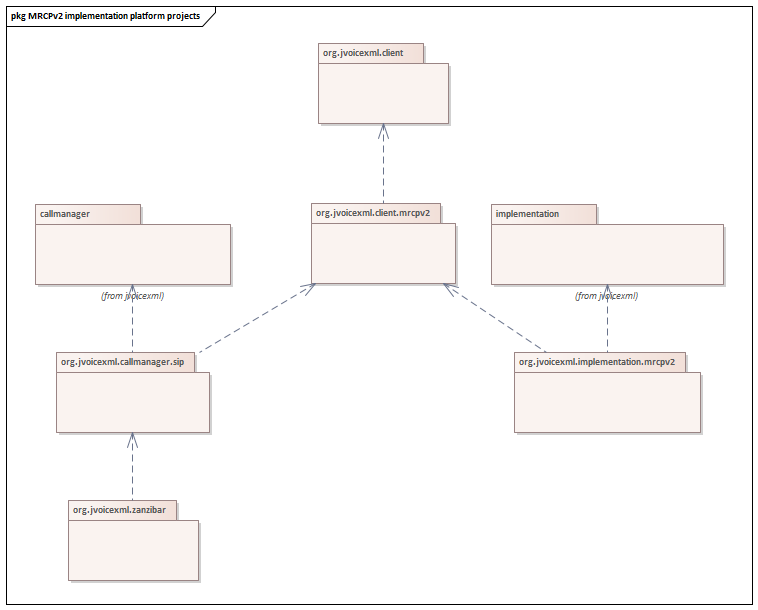
\includegraphics[width=\linewidth]{MRCPv2-implementation-platform-projects.png}
\caption{MRCPv2 Implementation Platform Projects}
\label{fig:MRCPv2-implementation-platform-projects}
\end{figure}

\subsubsection{Depending Subprojects}

This implementation plaform depends on the following projects.
\begin{itemize}
\item \texttt{org.jvoicexml.client.mrcpv2}
\item \texttt{org.jvoicexml.callmanager.sip}
\end{itemize}

\subsubsection{Project Specific Configuration}

The project settings for this subproject can be adapted by the following
properties in your copy of the \texttt{gradle.properties} file in the
\texttt{\${HOME}/.gradle} folder of the core project (see 
Appendix~\ref{sec:gradle-properties}):
\begin{lstlisting}
JVOICEXML_IMPLEMENTATION_MRCPV2 = false
JVOICEXML_IMPLEMENTATION_MRCPV2_SIP_ADDRESS = sip:cairogate@127.0.0.1
JVOICEXML_IMPLEMENTATION_MRCPV2_SIP_PORT = 5090
JVOICEXML_IMPLEMENTATION_MRCPV2_CAIRO_ADDRESS = sip:cairo@127.0.0.1
JVOICEXML_IMPLEMENTATION_MRCPV2_CAIRO_HOST = 127.0.0.1
JVOICEXML_IMPLEMENTATION_MRCPV2_CAIRO_PORT = 15050
JVOICEXML_IMPLEMENTATION_MRCPV2_CAIRO_BASE_RCV_RTP_PORT = 42150
JVOICEXML_IMPLEMENTATION_MRCPV2_CAIRO_BASE_XMIT_RTP_PORT = 42050
\end{lstlisting}

\subsubsection{Implementation Platform Configuration Files}

At runtime, this platform will be enabled if the following configuration file is found in the configuration
folder
\begin{itemize}
\item mrcpv2-implementation.xml
\end{itemize}

\subsubsection{Project \texttt{org.jvoicexml.callmanager.sip}}

Call manager for the MRCPv2 implementation platform which will be built in case this implementation platform is enabled.

\paragraph{Implementation Platform Configuration Files}

At runtime, this platform will be enabled if the following configuration file is found in the configuration
folder
\begin{itemize}
\item sip-callmanager.xml
\end{itemize}
 
\subsubsection{Project \texttt{org.jvoicexml.client.mrcpv2}}

Client configuration files used by the MRCPv2 implementation platform and the SIP call manager.

\subsection{Project \texttt{org.jvoicexml.implementation.text}}
\label{sec:text-implemenation-platform}

The text based implementation platform provides a text based input and output.
This means that you receive the system output as Java strings and you are able
to provide input via Java strings.

The text implementation platform comprises several projects as shown in figure~\ref{fig:text-implementation-platform-projects}.
\begin{figure}
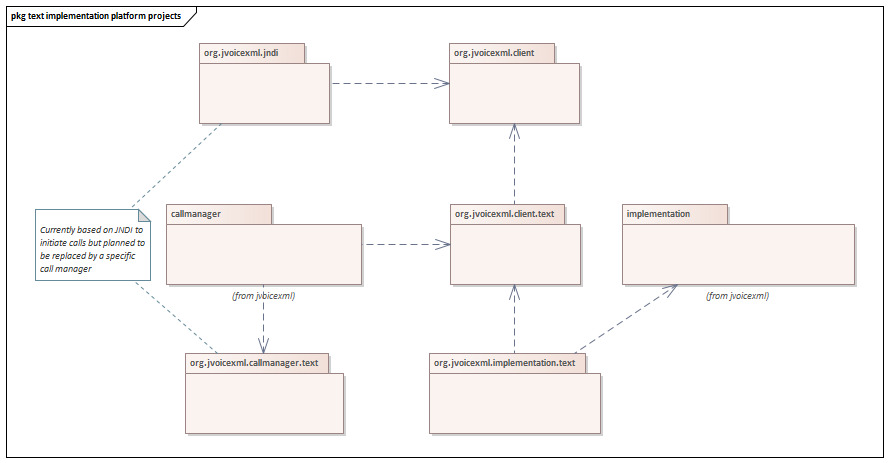
\includegraphics[width=\linewidth]{text-implementation-platform-projects.png}
\caption{Text Implementation Platform Projects}
\label{fig:text-implementation-platform-projects}
\end{figure}

\subsubsection{Depending Subprojects}

This implementation plaform depends on the following projects.
\begin{itemize}
\item \texttt{org.jvoicexml.client.txt}
\item \texttt{org.jvoicexml.callmanager.text}
\end{itemize}

\subsubsection{Project Specific Configuration}

The project settings for this subproject can be adapted by the following 
properties in your copy of the \texttt{gradle.properties} file in the
\texttt{\${HOME}/.gradle} folder of the core project (see 
Appendix~\ref{sec:gradle-properties}):

\begin{description}
\item[JVOICEXML\_IMPLEMENTATION\_TEXT] A value of \texttt{true} will enable this implementation
platform.
\end{description}

\paragraph{Implementation Platform Configuration Files}

At runtime, this platform will be enabled if the following configuration file is found in the configuration
folder
\begin{itemize}
\item text-implementation.xml
\end{itemize}

\subsubsection{Project \texttt{org.jvoicexml.callmanger.text}}

This callmanager aims at accessing JVoiceXML as a server for text based
access under development. In contrast to the text based implementation platform this callmanager
does not require JNDI.

\paragraph{Project Specific Configuration}

The project settings for this subproject currently does not support adaptation by the following
properties

\subsubsection{Project \texttt{org.jvoicexml.client.text}}

Client configuration files used by the text implementation platform and the text call manager.

\section{Document Server}

A document server provides access for JVoiceXML to VoiceXML documents, grammar files and 
other related documents.

\subsection{Project \texttt{org.jvoicexml.documentserver.jetty}}

This document server provides a small document repository based on Jetty. A document repository 
might be used for storing intermediate documents that are generated while processing a VoiceXML document.

\subsubsection{Project Specific Configuration}

The project settings for this subproject currently does not support adaptation.

\paragraph{Implementation Platform Configuration Files}

At runtime, this platform will be enabled if the following configuration file is found in the configuration
folder
\begin{itemize}
\item jetty-documentrepository.xml
\end{itemize}

\subsection{org.jvoicexml.documentserver.schemestrategy.file}

Support to access file based resources.

\subsubsection{Project Specific Configuration}

The project settings for this subproject currently does not support adaptation.

\paragraph{Implementation Platform Configuration Files}

At runtime, this platform will be enabled if the following configuration file is found in the configuration
folder
\begin{itemize}
\item file-schemestrategy.xml
\end{itemize}

\subsection{org.jvoicexml.documentserver.schemestrategy.http}

Support to access HTTP and HTTPS based resources.

\subsubsection{Project Specific Configuration}

The project settings for this subproject currently does not support adaptation.

\paragraph{Implementation Platform Configuration Files}

At runtime, this platform will be enabled if one of the following configuration files is found in the configuration
folder
\begin{itemize}
\item http-schemestrategy.xml
\item https-schemestrategy.xml
\end{itemize}

\section{Data Model}

The data model is a repository for both user- and system-defined data and properties.
The data model API does not assume any particular underlying
representation of the data or any specific access language, thus allowing
implementations to plug in different concrete data model languages.


\subsection{Project \texttt{org.jvoicexml.interpreter.datamodel.ecmascript}}

A data model based on ECMAscript.

\subsubsection{Project Specific Configuration}

The project settings for this subproject currently does not support adaptation.

\paragraph{Implementation Platform Configuration Files}

At runtime, this platform will be enabled if the following configuration file is found in the configuration
folder
\begin{itemize}
\item ecmascript-datamodel.xml
\end{itemize}

\section{Grammars}

JVoiceXML ships with the following grammar beyond what is defined in the VoiceXML specification~\cite{w3.org:voicexml}.


\subsection{Project \texttt{org.jvoicexml.interpreter.grammar.luis}}

\subsubsection{Project Specific Configuration}

A grammar extension to communicate with Microsoft LUIS.

\paragraph{Implementation Platform Configuration Files}

At runtime, this platform will be enabled if the following configuration file is found in the configuration
folder
\begin{itemize}
\item luis-grammar.xml
\end{itemize}

\subsection{Project \texttt{org.jvoicexml.interpreter.grammar.regex}}

\subsubsection{Project Specific Configuration}

A grammar extension to use regulare expressions as grammar.

\paragraph{Implementation Platform Configuration Files}

At runtime, this platform will be enabled if the following configuration file is found in the configuration
folder
\begin{itemize}
\item regex-grammar.xml
\end{itemize}

\section {MMI Support}

\subsection{Project \texttt{org.jvoicexml.callmanger.mmi}}

This callmanager allows for accessing JVoiceXML as a modality component in
the W3C MMI architectural pattern~\cite{w3c:2012:mmi_arch}.

The MMI support comprises several projects as shown in figure~\ref{fig:MMI-projects}.
\begin{figure}
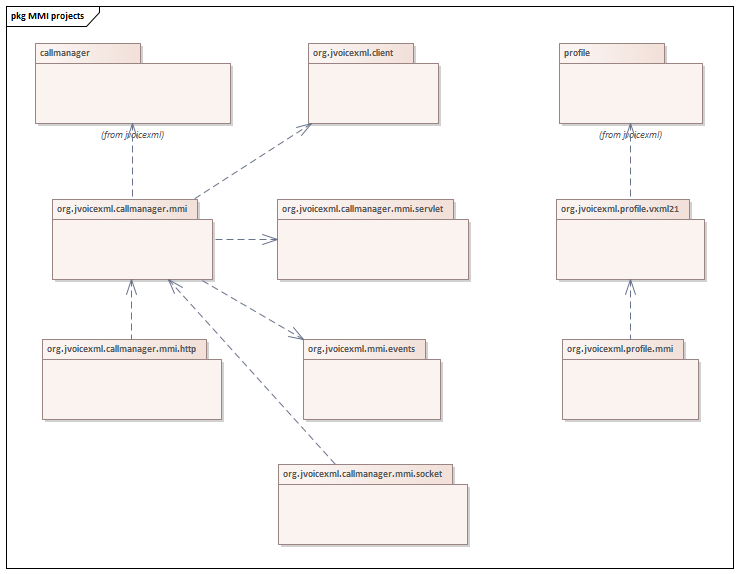
\includegraphics[width=\linewidth]{MMI-projects.png}
\caption{MMI Projects}
\label{fig:MMI-projects}
\end{figure}

\subsubsection{Project Specific Configuration}

The project settings for this subproject can be adapted by the following 
properties in your copy of the \texttt{gradle.properties} file in the
\texttt{\${HOME}/.gradle} folder of the core project (see 
Appendix~\ref{sec:gradle-properties}):

\begin{description}
\item[JVOICEXML\_PROFILE\_MMI] A value of \texttt{true} will enable MMI support.
\item[JVOICEXML\_PROFILE\_MMI\_HTTP] A value of \texttt{true} will use HTTP as ETL
\item[JVOICEXML\_PROFILE\_MMI\_SOCKET] A value of \texttt{true} will use sockets as ETL
\end{description}

\subsection{Project \texttt{org.jvoicexml.mmi.http}}

This project contains an implementation of the Event and Transport Layer
via HTTP. MMI events are received as XML.


\subsection{Project \texttt{org.jvoicexml.mmi.socket}}

This project contains an implementation of the Event and Transport Layer
via sockets. MMI events are received as XML.


\subsection{Project \texttt{org.jvoicexml.callmanager.mmi.servlet}}
\label{sec:mmi-servlet}

This project adds support for VoiceXML snippets that can be received
in the \lstinline{Content} attributes of the \lstinline{PrepareRequest}
or \lstinline{StartRequest} of the MMI events.

The resulting web archive must be deployed manually to a servlet container
of your choice (see section \ref{sec:tomcat}).


\subsection{Project \texttt{org.jvoicexml.mmi.events}}
\label{sec:mmi-events}

This project is a library to author MMI compatible events that can be used in
the MMI architectural pattern from the W3C.

Currently the library is able to generate events in XML format and for
protobuf~\cite{google:protobuf}. 

\section{Demo Programs}

The demo programs give a short impression how the JVoiceXML voice browser can
be used.

The demos comprise the following sub-projects:

\begin{description}
\item[org.jvoicexml.demo.embedded] A demo project that shows how JVoiceXML can
be embedded into other projects.
\item[org.jvoicexml.demo.helloworlddemo] The venerable hello world in Voice\-XML
\item[org.jvoicexml.demo.helloworldservletdemo] The same but as a servlet
\item[org.jvoicexml.demo.inputdemo] A small cinema application
\item[org.jvoicexml.demo.jtapidemo] SIP based access to JVoiceXML calling the
hello world servlet demo (not functional)
\item[org.jvoicexml.demo.mixedinitiativedemo] Demo to show how the mix\-ed
initiative capabilities.
\item[org.jvoicexml.mmi.simpledemo] Demo to show MMI capabilities.
\item[org.jvoicexml.demo.objecttagdemo] Demo to show how the object tag can be
used.
\item[org.jvoicexml.demo.recorddemo] Demo for the record tag
\item[org.jvoicexml.demo.scriptdemo] Demo for scripting functionality with a
weird dialog flow
\item[org.jvoicexml.demo.simpleinputdemo] A simple input demo
\item[org.jvoicexml.demo.subdialogdemo] Demo to show a subdialog
\item[org.jvoicexml.demo.talkingheaddemo] Demo to show the talking head in action
\item[org.jvoicexml.demo.textdemo] Demo to show how to use the text platform
\item[org.jvoicexml.demo.voicexmlcreationdemo] Demo for the VoiceXML XML library
\end{description}

\section{Eclipse Plug in}

The eclipse plug-in allows to run JVoiceXML as a server from within the eclipse
IDE and to start VoiceXML sessions from eclipse.

\begin{description}
\item[org.jvoicexml.eclipse.debug.ui] Basic UI Widgets for VoiceXML debugging
\item[org.jvoicexml.eclipse.debug.ui.launching] Eclipse plug-in as a basic
framework for VoiceXML debugging
\item[org.jvoicexml.eclipse.debug.ui.launching.jvoicexml] Implementation of the
basic framework for JVoiceXML
\item[org.jvoicexml.eclipse.jst.server] Eclipse plug-in to start the JVoiceXML
server from the eclipse server view
\item[org.jvoicexml.eclipse.features] Eclipse features for the JVoiceXML
plug-in.
\item[org.jvoicexml.eclipse.updatesite] Eclipse update site for the
JVoiceXML plug-in
\end{description}

\section{VoiceXML Unit}
\label{voicexml-unit}

This component is an approach to establish unit testing capabilities for
VoiceXML. VoiceXML unit makes use of the text implementation platform~\ref{sec:text-implemenation-platform}.

It consists of the following projects
\begin{description}
\item[org.jvoicexml.voicexmlunit] VoiceXML unit test framewortk
\item[org.jvoicexml.voicexmlunit.demo] Demo test project
\end{description}

\subsubsection{Project Specific Configuration}

The project settings for this subproject currently does not support adaptation.

\section{System test}

The system test implements the W3C's conformance test for VoiceXML 2.1.

In addition you will need the following sub-projects:
\begin{itemize}
\item org.jvoicexml
\item org.jvoicexml.xml
\item org.jvoicexml.client
\item org.jvoicexml.client.text
\item org.jvoicexml.implementation.text
\end{itemize} 

\section{Documentation}

The documentation comprise the following sub-projects:

\begin{description}
\item[howtobuild] The how to build JVoiceXML documentation (this document)
\item[userguide] A tutorial to start working with JVoiceXML
\end{description}

Both guides are written in \LaTeX and you will need to have a \LaTeX compiler
installed. For Windows, MiKTeX as mentioned above is an option.


\section{Code Conventions}
\label{sec:code-conventions}

We follow the JAVA code conventions~\cite{sun:codeconv} for our code. All
methods and member variables must be commented using 
JAVADOC~\cite{sun:javadoc_guidelines}.

In addition we use a \texttt{TODO} tag to mark sections that need further work.

Example:

\begin{lstlisting}[language=Java]
// TODO Implement the untreated case XYZ
\end{lstlisting}

We use checkstyle~\cite{checkstyle} to check our coding conventions.
All developers are requested to execute the \emph{checkstyle} target
of our ANT buildfile, see section~\ref{sec:main-build-file}. 
There are plug-ins for some IDEs, which you can use if you want to. The
\texttt{checkstyle.xml} can be found in the folder 
\texttt{etc} and is called \texttt{jvoicexml-checks.xml}.

With the help of the checkstyle plugin these tests can be run automatically
and visualized inside eclipse. Therefore, each project has to be configured to
use this project relative configuration file. A screenshot is shown inside
figure~\ref{fig:eclipse-project-checkstyle}.
\begin{figure}
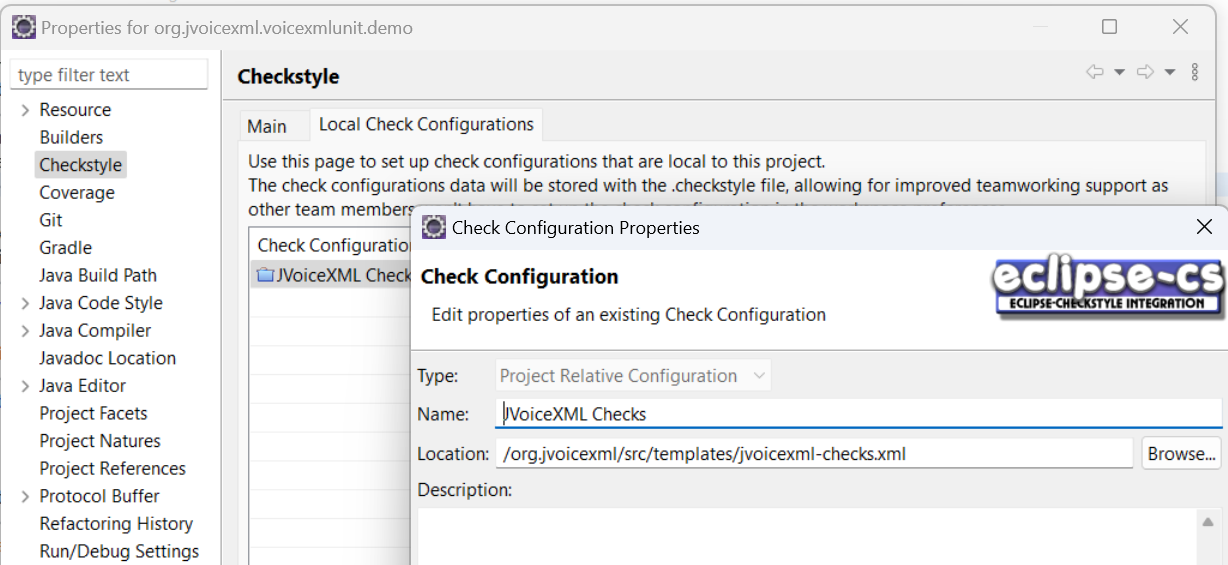
\includegraphics[width=\linewidth]{eclipse-project-checkstyle.png}
\caption{Project relative configuration of checkstyle within eclipse}
\label{fig:eclipse-project-checkstyle}
\end{figure}


Developers are requested to use the \texttt[language=Java]{@inheritDoc}
JAVADOC tag in favor of a \texttt[language=Java]{@see} reference for inherited documentation.
Pros of the \texttt[language=Java]{@inheritDoc} tag, taken 
from~\cite{tauber:inheritdoc}, are
\begin{itemize}
\item satisfies checkstyle requirements for JAVADOC,
\item no references to go stale,
\item additional doc specific to this implementation will appear in JAVADOC and
\item inherited doc in JAVADOC.
\end{itemize}

All source files must contain the following header about the 
copyright, see section~\ref{sec:copyright}, that we use for JVoiceXML.

\begin{lstlisting}[language=Java]
/*
 * JVoiceXML - A free VoiceXML implementation.
 *
 * Copyright (C) 2015 JVoiceXML group - 
 *      http://jvoicexml.sourceforge.net
 *
 * This library is free software; you can redistribute it 
 * and/or modify it under the terms of the GNU Library 
 * General Public License as published by the Free Software 
 * Foundation; either version 2 of the License, or (at your 
 * option) any later version.
 *
 * This library is distributed in the hope that it will be 
 * useful, but WITHOUT ANY WARRANTY; without even the 
 * implied warranty of MERCHANTABILITY or FITNESS FOR A 
 * PARTICULAR PURPOSE.  See the GNU Library General Public 
 * License for more details.
 *
 * You should have received a copy of the GNU Library 
 * General Public License along with this library; if 
 * not, write to  the Free Software Foundation, Inc., 
 * 59 Temple Place, Suite 330, Boston, MA  02111-1307  USA
 *
 */
\end{lstlisting}

The class comment has to contain the following information:

\begin{lstlisting}[language=Java]

/**
 * Comment about the purpose of this class.
 *
 * @author <Name of the author>
 * @author <Other authors>
 * @since <current version number>
 */
\end{lstlisting}

The name of the author and the purpose have to be replaced by their proper
values.

\section{Releases}

This section describes the required steps to create a new release for
JVoice\-XML.
Before you start make sure that Java 8 is used as the default JVM.

\subsection{Creation of a Release Workspace}

New releases are \emph{never} built from the workspace to ensure that there are
no changes in the workspace that are not reflected in the SVN repository.
Therefore change to an empty directory and do a fresh checkout.


\subsection{Unit Tests}

There are many unit tests based on JUnit to ensure the correctness of the
classes written for JVoiceXML. Some tests need customized settings, e.g. to
start the Mary TTS server. These settings are maintained in your local copy of the
\texttt{gradle.properties}.

Open a command prompt at this directory and call
\begin{lstlisting}
gradelw testClasses
\end{lstlisting}

After the tests are finished. There must not be any errors or failures in the summary. Note that
some tests require an active Internet connection. 

If you detect any errors correct identify the cause for it, correct them
yourself or contact the responsible developer of the module. After the errors
have been fixed, restart from the beginning to make a new release.

\subsection{Create the Distribution}

After the unit test ran successfully, the binary distribution can be built.
Update the version number in the project's \texttt{gradle.properties}
and comment the version number in you local copy of this file.The JVoiceXML version number consists of
\begin{lstlisting}
 <major-version>.<minor-version>[-SNAPSHOT]
\end{lstlisting}

Create a distribution configuration by calling
\begin{lstlisting}
gradelw :main:distZipt
\end{lstlisting}

\subsection{Test the Installation}

Unpack the distribution into a new folder
Select all available packages and test the installation. 
Start the voice browser and check if there are any errors in the log when
JVoiceXML starts.

Uninstall JVoiceXML and reinstall it with the JSAPI 1.0 implementation platform
only and the demos. Start JVoiceXML and check if all demos are working properly.
It should not be necessary to restart JVoiceXML while the demos are tested.

If any error occurs while testing, locate the cause of the error, fix it
yourself or identify the person who is responsible for the module and restart
the release process from the beginning.

\subsection{Tag the Release}

Commit the gradle properties file with the new version number.

The next step serves to tag the code of the release version. 

\subsection{Upload the Distribution}

Uplaod the release to the GitHub home page.

\subsection{Prepare the Further Development}

Prepare the next version by incrementing the version number in the project's Gradle
properties file  and committing that file.

\subsection{Creation of Snapshots for Maven}

Some subprojects are ready to be upload snapshots for Maven to
Sonatype\footnote{\url{http://www.sonatype.com}}. Sonatype offers
a free repository hosting service using Nexus for open soource projects.

Therefore deployers are requested to sign up for their servie. Detailed
instructions are given at \url{https://docs.sonatype.org/display/Repository/Sonatype+OSS+Maven+Repository+Usage+Guide}.

Prepare values for the following properties in your local copy of the Gradle properties.

\begin{lstlisting}[language=XML]
# Settings for signing
# Currently, signing does not work with PGP 2.1 and newer
signing.keyId = PGP_SIGNING_KEY
signing.password = PGP_SIGNING_PASSWORD
signing.secretKeyRingFile = PGP_SECRET_KEY_RING

# Sonatype credentials
JVOICEXML_OSSRH_USERNAME=MUST-BE-SUPPLIED-VALUE
JVOICEXML_OSSRH_PASSWORD=MUST-BE-SUPPLIED-VALUE
\end{lstlisting}

Afterwards call 
\begin{lstlisting}
gradelw publish
\end{lstlisting}

The snapshots will use the SVN version number to differentiate between different
snapshots of the same jar. Consequently, you will have to have at least
a commit between two snapshots.

\bibliography{howtobuild}
\bibliographystyle{plain}

\newpage

\appendix

\section{gradle.properties}
\label{sec:gradle-properties}

Customizable settings of JVoiceXML. Create a copy of this file in the
\texttt{\$HOME/.gradle} folder for local modifications.

\lstinputlisting{../gradle.properties}

\end{document}

% LocalWords:  JVoiceXML VoiceXML APIs JSAPI JTAPI mkdir cd CVS SourceForge cvs
% LocalWords:  pserver CVSROOT acls RSH lll xml LGPL src api JAVADOC rdparty XP
% LocalWords:  IDE jvoicexml dir JCP JSR jsapi BCL chmod FreeTTS TTS freetts
% LocalWords:  jvxml impl todo XYZ checkstyle Schnelle howtobuild basicstyle
% LocalWords:  RFE numberstyle stepnumber kkv href Revison JVoice Adrindam Das
% LocalWords:  TortoiseCVS cygwin  CMU tex schnelle WSJ gau dCep mel Mozilla
% LocalWords:  projecthelp backgroundcolor lightgray subfolder lang buildfile
% LocalWords:  plugins IDEs inheritDoc inhe rit RCSfile login apidoc loggings
% LocalWords:  distributionFolder IDE's Ingimar SVN svn trunc HTTPS config RTP
% LocalWords:  CLASSPATH GJTAPI jlibrtp JainSIP gjtapi HeadURL LastChangedDate
% LocalWords:  LastChangedRevision LastChangedBy propset
